% biography section
% 
% If you have an EPS/PDF photo (graphicx package needed) extra braces are
% needed around the contents of the optional argument to biography to prevent
% the LaTeX parser from getting confused when it sees the complicated
% \includegraphics command within an optional argument. (You could create
% your own custom macro containing the \includegraphics command to make things
% simpler here.)
%\begin{IEEEbiography}[{\includegraphics[width=1in,height=1.25in,clip,keepaspectratio]{mshell}}]{Michael Shell}
% or if you just want to reserve a space for a photo:
\begin{IEEEbiography}[{
		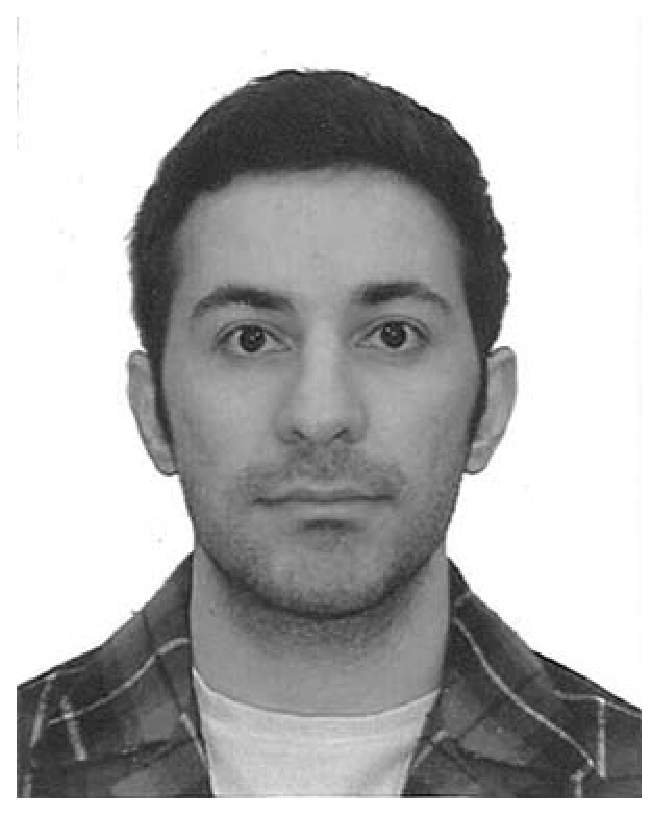
\includegraphics[width=1in,height=1.25in,clip,keepaspectratio]{figs/mohammadi.eps}
	}]{Ali Mohammadi Teshnizi}
	(Student Member, IEEE) received the B.S. degree in computer engineering from
	University of Tehran in 2020. He is currently pursuing the M.S. degree in computer science with University of Calgary, where he is a Research
	Assistant. His research interests include the applications of machine learning and deep learning, radio communications and network security, and the Internet of Things (IoT).
\end{IEEEbiography}
\vskip-1.5 \baselineskip
\begin{IEEEbiography}
	[{
	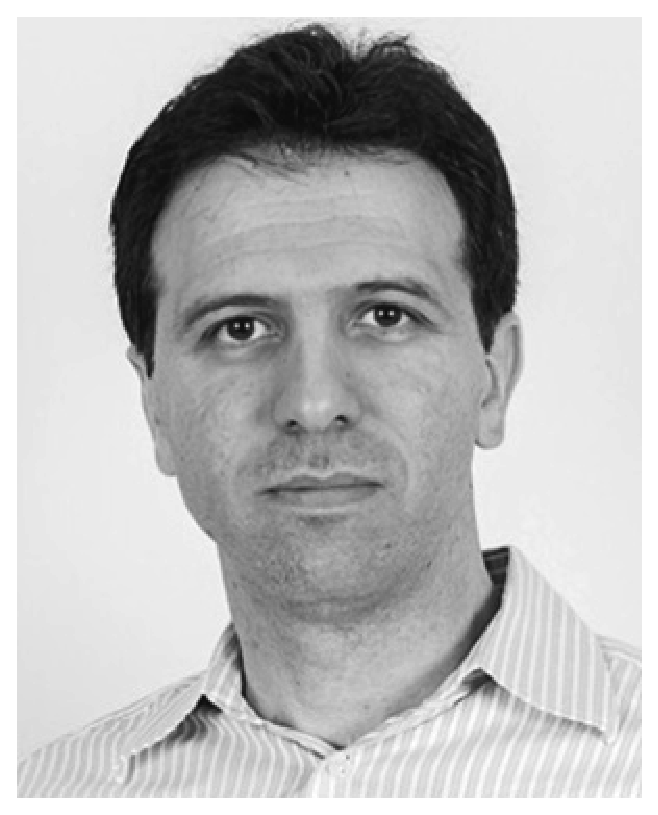
\includegraphics[width=1in,height=1.25in,clip,keepaspectratio]{figs/ghaderi.eps}
	}]{Majid Ghaderi}
(Member, IEEE) received the B.Sc. and M.Sc. degrees in computer science from the Sharif University of Technology and the Ph.D. degree in computer science from the University of Waterloo. He is a Professor with the Computer Science Department, University of Calgary. His general area of research is computer networks. In the broader context of computer networks, his current research focus is on: design and optimization of network algorithms, secure communication in networked systems, and Application of machine learning in network control. The unifying theme of his research is the fusion of theoretical research with real-world applications in the computer networking area.
\end{IEEEbiography}
\vskip-2.5\baselineskip
\begin{IEEEbiography}[{
		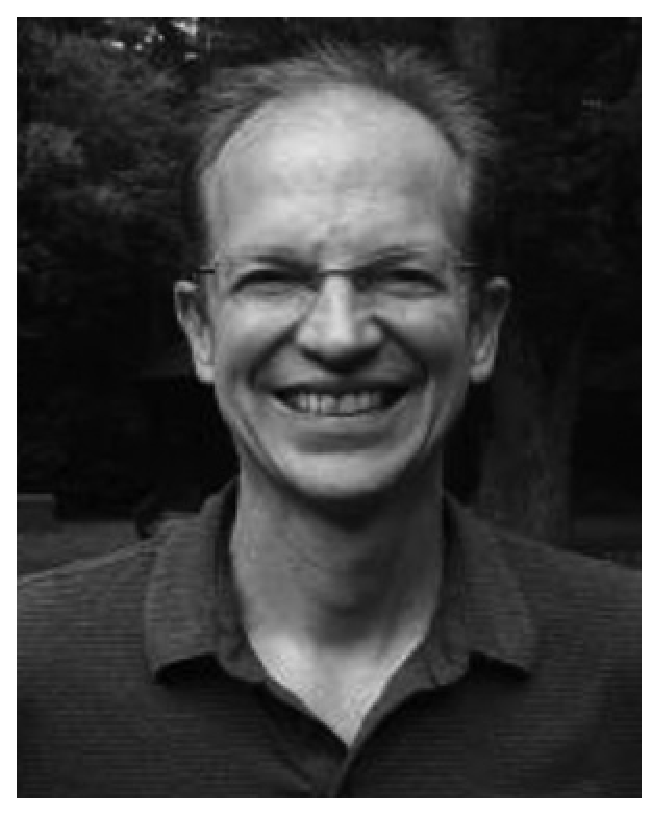
\includegraphics[width=1in,height=1.25in,clip,keepaspectratio]{figs/goeckel.eps}
	}]{Dennis Goeckel}
(Fellow, IEEE) received the B.S. degree from Purdue University, West Lafayette, IN, USA, in 1992, and the M.S. and Ph.D. degrees from the University of Michigan, Ann Arbor, MI, USA, in 1993 and 1996, respectively.,Since 1996, he has been with the ECE Department, University of Massachusetts at Amherst, Amherst, MA, USA, where he is currently a Professor. Prof. Goeckel received the University of Massachusetts Distinguished Teaching Award in 2007. He received the NSF CAREER Award in 1999 and is an IEEE Fellow for ``contributions to wireless communication systems and networks''. He was a Lilly Teaching Fellow from 2000 to 2001.
\end{IEEEbiography}

% if you will not have a photo at all:
%\begin{IEEEbiographynophoto}{John Doe}
%	Biography text here.
%\end{IEEEbiographynophoto}

% insert where needed to balance the two columns on the last page with
% biographies
%\newpage

%\begin{IEEEbiographynophoto}{Jane Doe}
%	Biography text here.
%\end{IEEEbiographynophoto}

% You can push biographies down or up by placing
% a \vfill before or after them. The appropriate
% use of \vfill depends on what kind of text is
% on the last page and whether or not the columns
% are being equalized.

%\vfill

% Can be used to pull up biographies so that the bottom of the last one
% is flush with the other column.
%\enlargethispage{-1in}